\section{Patrón de Diseño Bridge} 
\textbf{}\\
Es normalmente uno de los patrones que más cuesta entender, especialmente si nos ceñimos únicamente a su descripción. La idea tras este patrón, sin embargo, es sencilla: dado que cualquier cambio que se realice sobre una abstracción afectará a todas las clases que la implementan, Bridge propone añadir un nuevo nivel de abstracción entre ambos elementos que permitan que puedan desarrollarse cada uno por su lado.
\begin{flushleft}
\begin{center}
	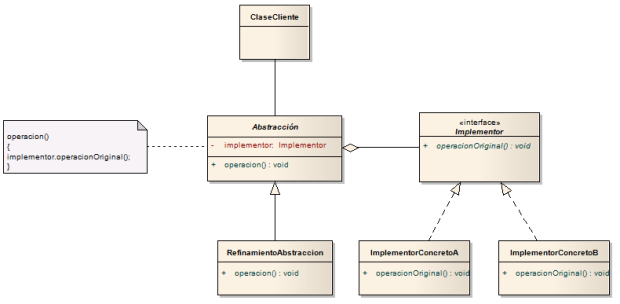
\includegraphics[width=10cm]{./Imagenes/bridge1} 
	\end{center}
\begin{itemize}


\textbf {1.	¿Por qué “Bridge”?}
\textbf{}\\
Patrón tras patrón, vemos que los mismos conceptos se repiten una y otra vez. Minimizar el acoplamiento, hacer que las clases dependan de abstracciones en lugar de depender de implementaciones, preferir el uso de composición antes que el uso de herencia… El patrón Bridge no es una excepción. Sin embargo, hasta el momento todos los patrones que hemos visto tenían una relación entre su nombre y su funcionalidad. Un Adapter adapta. Una factoría fabrica objetos. Un Builder construye. Pero… ¿Bridge? ¿Qué tiene que ver un puente con todo esto?
\textbf{}\\
Una de las razones por las que opino que este patrón es complicado de entender a la primera es, precisamente, que no existe una relación clara entre su nombre y su descripción. ¿Llamar puente a desligar una interfaz de la implementación? ¿Por qué? La razón no está tanto en este proceso sino en el camino que existe entre la clase que refina la abstracción y las implementaciones de la interfaz.
\textbf{}\\
Hablando en plata, y a modo de resumen, realizaremos la transformación del siguiente árbol de herencia:


\begin{center}
	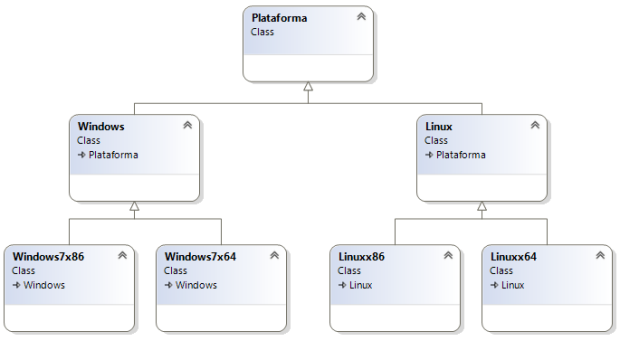
\includegraphics[width=10cm]{./Imagenes/bridge2} 
	\end{center}

\textbf{}\\
En una composición como la siguiente:
\begin{center}
	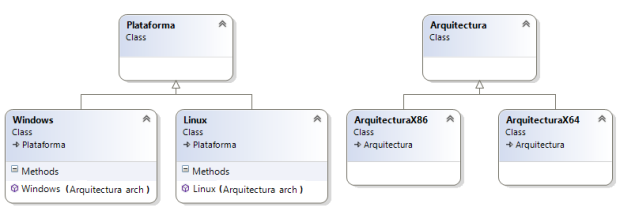
\includegraphics[width=10cm]{./Imagenes/bridge3} 
	\end{center}

\textbf {2.	Similitudes}
\textbf{}\\

La estructura de este patrón se parece mucho a la del patrón Adapter, ya que nuestra clase Abstracción hace las veces de “adaptador” entre nuestra clase cliente y la interfaz Implementor. Sin embargo, nos movemos por la sinuosa senda de la ingeniería, por lo que afirmar que Adapter y Bridge realizan lo mismo simplemente porque su estructura sea muy parecida es quedarnos en la superficie del problema que tratamos de resolver.
La estructura de este patrón se parece mucho a la del patrón Adapter, ya que nuestra clase Abstracción hace las veces de “adaptador” entre nuestra clase cliente y la interfaz Implementor. Sin embargo, nos movemos por la sinuosa senda de la ingeniería, por lo que afirmar que Adapter y Bridge realizan lo mismo simplemente porque su estructura sea muy parecida es quedarnos en la superficie del problema que tratamos de resolver.

\item \textbf {Un ejemplo de patrón Bridge}
\textbf{}\\

Veamos la aplicación de nuestro patrón Bridge con un ejemplo en código C sharp. El ejemplo, como seguro que habréis adivinado, estará basado en vehículos. Nuestra abstracción simbolizará el vehículo en sí, mientras que la parte que se tenderá “al otro lado del puente” será el motor del mismo. Los tipos de vehículo podrán así evolucionar con independencia de los motores que éstos posean.
Comenzaremos codificando la interfaz Implementor, que en nuestro ejemplo estará representada por el motor. O más específicamente, por la interfaz IMotor.
\begin{center}
\textbf {MOTOR}
	\end{center}

\begin{center}
	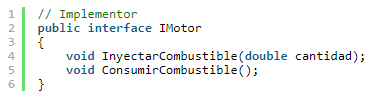
\includegraphics[width=10cm]{./Imagenes/bridge4} 
	\end{center}

Como vemos, nada complicado: nuestro Implementor expone dos métodos, InyectarCombustibley ConsumirCombustible, que deberán ser codificados en las clases que implementen la interfaz. Y dicho y hecho, añadiremos un par de clases cuyo papel en el patrón se corresponderá con ImplementorConcretoA e ImplementorConcretoB, y modelarán dos tipos de motores: diesel y gasolina.
\textbf{}\\

\begin{center}
\textbf {DIESEL}
	\end{center}

\begin{center}
	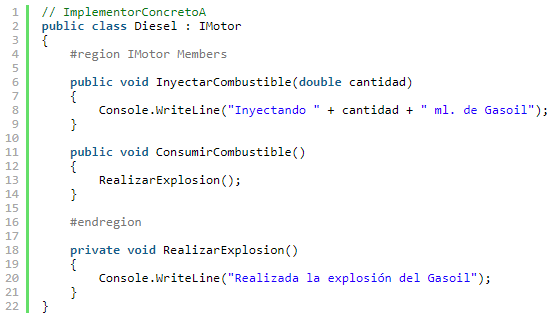
\includegraphics[width=10cm]{./Imagenes/bridge5} 
	\end{center}

\textbf{}\\
\begin{center}
\textbf {GASOLINA}
	\end{center}

\begin{center}
	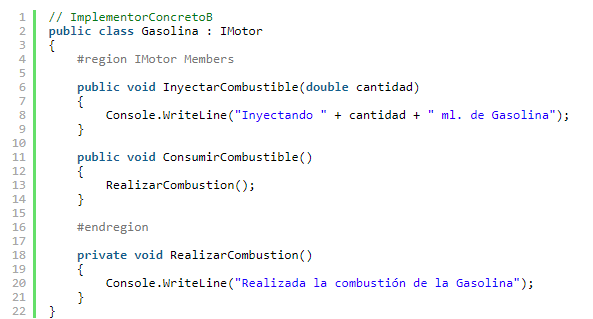
\includegraphics[width=10cm]{./Imagenes/bridge6} 
	\end{center}

Con estas tres clases ya habríamos desarrollado el subárbol izquierdo del diagrama UML que mostramos al comienzo del artículo: la interfaz Implementor junto a sus implementaciones:

\textbf{}\\
\begin{center}
	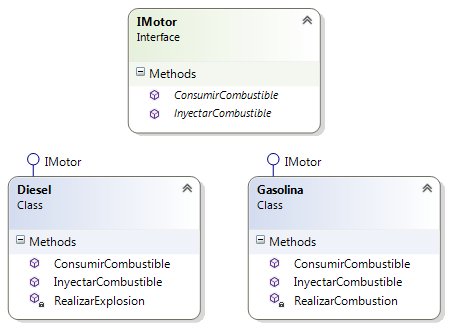
\includegraphics[width=10cm]{./Imagenes/bridge7} 
	\end{center}

La siguiente parte será encapsular la interfaz dentro de nuestra abstracción Vehiculo, que dispondrá de una referencia a IMotor y de un método que hará uso de los métodos de nuestra interfaz, encapsulando su funcionalidad tal y como hacíamos en el patrón Adapter:
\textbf{}\\
\begin{center}
\textbf {VEHICULO}
	\end{center}

\begin{center}
	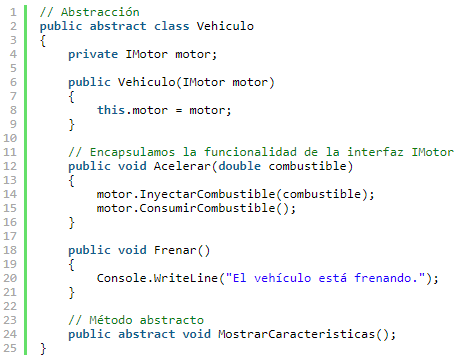
\includegraphics[width=10cm]{./Imagenes/bridge8} 
	\end{center}

Como venimos observando a lo largo de los últimos patrones, el objeto que implementará el motor es inyectado en el constructor, siguiendo el quinto de los principios SOLID.
\textbf{}\\
Por último, codificaremos la evolución de nuestra abstracción, que se corresponderá con RefinamientoAbstracciónA y RefinamientoAbstracciónB, representadas por dos tipos de vehículos: Berlina y Monovolumen.

\textbf{}\\
\begin{center}
\textbf {VERLINA}
	\end{center}

\begin{center}
	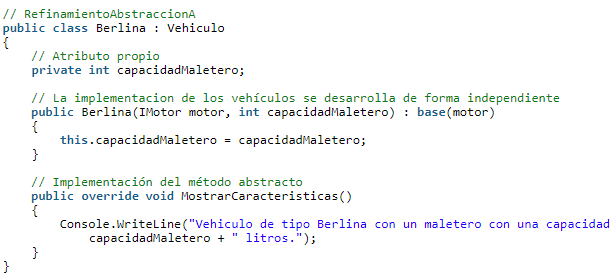
\includegraphics[width=10cm]{./Imagenes/bridge9} 
	\end{center}
\textbf{}\\
\textbf{}\\
\textbf{}\\
\textbf{}\\
\textbf{}\\
\textbf{}\\
\textbf {3.	¿Cuándo utilizar este patrón?}
\textbf{}\\
Un ejemplo típico de un patrón Bridge lo puede conformar cualquier familia de drivers de un dispositivo, tal y como vimos en el primer ejemplo.
\textbf{}\\
Otro ejemplo típico suele ser el de las APIs de dibujo. Los elementos genéricos, tales como formas y figuras serían las abstracciones (por ejemplo, Forma sería el elemento Abstraction del que derivarían abstracciones refinadas como Circulo o Cuadrado), mientras que la parte “dependiente” del sistema sería la API concreta que se encargaría de dibujar en pantalla las formas genéricas definidas en la abstracción. Este funcionamiento puede observarse en los paquetes de java java.awt y java.awt.peer. (en Button y List, por ejemplo).
\textbf{}\\
Las situaciones óptimas en los que se debe utilizar este patrón serán, por tanto:

\item Cuando se desea evitar un enlace permanente entre la abstracción y (toda o parte de) su implementación.
\item Cuando los cambios en la implementación de una abstracción no debe afectar a las clases que hace uso de ella.
\item Cuando se desea compartir una implementación entre múltiples objetos.



	

\end{itemize} 


\end{flushleft}